\documentclass[oneside, 11pt]{article}

\usepackage[T1]{fontenc}
\usepackage[utf8]{inputenc}
\usepackage[dutch]{babel}

\usepackage{fouriernc}
\usepackage[detect-all, load-configurations=binary,
            separate-uncertainty=true, per-mode=symbol,
            retain-explicit-plus, range-phrase={ tot }]{siunitx}

\usepackage{setspace}
\setstretch{1.2}

\setlength{\parskip}{\smallskipamount}
\setlength{\parindent}{0pt}

\usepackage{geometry}
\geometry{marginparwidth=0.5cm, verbose, a4paper, tmargin=3cm, bmargin=3cm, lmargin=2cm, rmargin=2cm}

\usepackage{float}

\usepackage[fleqn]{amsmath}
\numberwithin{equation}{section}
\numberwithin{figure}{section}

\usepackage{graphicx}
\graphicspath{{Figures/}}
\usepackage{subfig}

\usepackage{tikz}
\usetikzlibrary{plotmarks}

\usepackage{fancyhdr}
\pagestyle{fancy}
\fancyhf{}
\rhead{\thepage}
\renewcommand{\footrulewidth}{0pt}
\renewcommand{\headrulewidth}{0pt}

\usepackage{relsize}
\usepackage{xspace}
\usepackage{url}

\newcommand{\figref}[1]{Figuur~\ref{#1}}

\newcommand{\hisparc}{\textsmaller{HiSPARC}\xspace}
\newcommand{\kascade}{\textsmaller{KASCADE}\xspace}
\newcommand{\sapphire}{\textsmaller{SAPPHiRE}\xspace}
\newcommand{\jsparc}{\textsmaller{jSparc}\xspace}
\newcommand{\hdf}{\textsmaller{HDF5}\xspace}
\newcommand{\aires}{\textsmaller{AIRES}\xspace}
\newcommand{\csv}{\textsmaller{CSV}\xspace}
\newcommand{\python}{\textsmaller{PYTHON}\xspace}
\newcommand{\corsika}{\textsmaller{CORSIKA}\xspace}
\newcommand{\labview}{\textsmaller{LabVIEW}\xspace}
\newcommand{\daq}{\textsmaller{DAQ}\xspace}
\newcommand{\adc}{\textsmaller{ADC}\xspace}
\newcommand{\adcs}{\textsmaller{ADC}s\xspace}
\newcommand{\Adcs}{A\textsmaller{DC}s\xspace}
\newcommand{\hi}{\textsc{h i}\xspace}
\newcommand{\hii}{\textsc{h ii}\xspace}
\newcommand{\mip}{\textsmaller{MIP}\xspace}
\newcommand{\hisparcii}{\textsmaller{HiSPARC II}\xspace}
\newcommand{\hisparciii}{\textsmaller{HiSPARC III}\xspace}
\newcommand{\pmt}{\textsmaller{PMT}\xspace}
\newcommand{\pmts}{\textsmaller{PMT}s\xspace}

\DeclareSIUnit{\electronvolt}{\ensuremath{\mathrm{e\!\!\:V}}}

\DeclareSIUnit{\unitsigma}{\ensuremath{\sigma}}
\DeclareSIUnit{\mip}{\textsmaller{MIP}}
\DeclareSIUnit{\adc}{\textsmaller{ADC}}

\DeclareSIUnit{\gauss}{G}
\DeclareSIUnit{\parsec}{pc}
\DeclareSIUnit{\year}{yr}


\usepackage{xfrac}
\usepackage{array}

\title{Bliksemonderzoek}
\author{C.G.N. van Veen}
\docrecept{1}{BO}
\version{1.0}

\begin{document}

\maketitle

\begin{tabular}{|c|c|}
\hline 
leerjaar & niveau \tabularnewline
\hline 
4/5 HAVO/VWO  & beginnend \tabularnewline
\hline 
\end{tabular}

\section{lesmateriaal}

Dit recept voor werken met \hisparc gaat in op het zoeken van correlaties tussen 
bliksem en kosmische showers. Het doel van deze lessenserie is om leerlingen 
kennis te laten maken met kosmische straling en ze een onderzoek te laten doen 
met de database van \hisparc, waarbij ze een correlatie proberen te vinden tussen 
bliksemontladingen en kosmische straling. Ze onderzoeken namelijk of er binnen een geschikt
tijdsinterval rond de bliksemontlading ook een kosmische shower (event) door 
een \hisparc station is gemeten.
Leerlingen krijgen eerst een introductie over kosmische straling en gaan
dan aan de slag met het analyseren van \hisparc data en in de laatste les kunnen 
de leerlingen onderzoeken en een verslag van hun bevindingen maken.
\\

\textbf{Alles wat nodig is voor deze lessenserie vindt u hier:}\\
\url{http://docs.hisparc.nl/zips/bliksemonderzoek.zip}


\textit{Bronnen:} Leerlingen kunnen tijdens deze lessenserie gebruik maken van de 
volgende websites:
1. Database met datum/posities van bliksemontladingen van het KNMI\\
\url{ http://www.knmi.nl/klimatologie/daggegevens/onweer/}

2. Achtergrond informatie bliksem en kosmischestraling (natuur en techniek)\\
\url{ http://bruno.home.xs4all.nl/2005/NWT%200705%20bliksem.pdf}

3. Zoeken in de database van \hisparc.\\
\url{http://data.hisparc.nl}\\
Klik op een station in de lijst, zodat je in het scherm van dat station komt.
Klik in dit nieuwe scherm op: \textit{Download event summary data}.
Voor verdere uitleg zie \figref{fig:overview_website} en \figref{fig:data_download}.

\vspace{5mm}

\begin{tabular}{|c|p{9cm}|c|}
\hline
lesnummer & lesdocument & bron \tabularnewline 
\hline
1 & Terminologie, Cosmic air showers, Werkblad: cosmic air showers, 
kosmische straling & Infopakket\tabularnewline
\hline
2 & Werken met data van \hisparc en KNMI & Website 1 en 3 \tabularnewline
\hline
3 & Zelfstandig onderzoek naar correlaties & Website 1 en 3 \tabularnewline
\hline
\end{tabular}

\section{Les 1}

Introductie van kosmische straling. In deze les starten we met
achtergrond materiaal en een werkblad. Belangrijk
is dat er een introductie op kosmische straling gegeven wordt en dat de
terminologie duidelijk wordt gemaakt.
Bij het laatste onderdeel kunnen leerlingen zelf informatie over bliksem zoeken.

\begin{itemize}
    \item Wat is kosmische straling?
    \item Hoe ontstaat een deeltjeslawine? 
    \item Hoe worden deze deeltjes in de lawine op aarde gedetecteerd?
    \item Hoe ontstaat bliksem? 
    \item Op welke gronden zou er een verband tussen bliksem en kosmische straling 
    kunnen zijn?
\end{itemize}

\textbf{Opmerking:}
Van de \hisparc site (\url{www.hisparc.nl}) kunnen diverse bestaande 
powerpoint-presentaties gedownload worden.
Deze presentaties mogen naar believen aangepast worden, om door 
leerlingen en docenten in de klas te gebruiken.

\section{Les 2}

In deze les leren de leerlingen hoe ze data van \hisparc en bliksem kunnen downloaden.
Het is ook van belang dat leerlingen dat leerlingen leren, de gedownloade `csv' bestanden
in te lezen in Excel. Daartoe kan de docent een voorbeeldbestand aanleveren.
Een online tutorial over inlezen van `csv' bestanden in Excel vindt U hier:\\
\url{ http://www.jkp-ads.com/Articles/importtextnl.asp} \\
De werkwijze om data te downloaden wordt in het kort uitgelegd in \figref{fig:overview_website}, 
\figref{fig:data_download}, \figref{fig:data_download_form} en \figref{fig:KNMI_data} van dit artikel.

In deze les behandelen we zaken als:
\begin{itemize}
    \item Hoe halen we data van de website van \hisparc?
    \item Hoe vinden we dagen met bliksem ontladingen?
    \item Hoe lezen we deze data uit met Excel?
\end{itemize}

Zoals te zien is in \figref{fig:KNMI_data}, is het relatief eenvoudig om dagen te vinden met 
bliksemdata.
\section{Les 3}

De leerlingen gaan in deze les aan de slag met de opdracht: "Kun je correlaties 
vinden tussen bliksemontlading en kosmische straling events?"

Gebruik bij deze les: het werkblad \textit{bliksem onderzoek} van het infopakket.
 
De docent is vrij om de leerlingen deze opdracht als oefening te laten doen of
een verslaglegging te vragen van de vorderingen van de leerlingen.

\section{Verdieping}

\begin{tabular}{|c|c|c|} 
\hline
leerdoelen & beschrijving bron & bron \tabularnewline
\hline
Datareconstructie met \hisparc & Lesmateriaal: Uitleg \hisparc & Infopakket\tabularnewline
\hline
\end{tabular}

\section{bronnen}

Materiaal voor lessen over kosmische stralingen is te vinden op de volgende websites:\\

\textbf{Infopakket} : \url{http://www.hisparc.nl/docent-student/lesmateriaal/informatie-pakket}

\textbf{Routenet} : \url{http://www.hisparc.nl/docent-student/lesmateriaal/routenetpad/} 

\begin{figure}
    \centering
    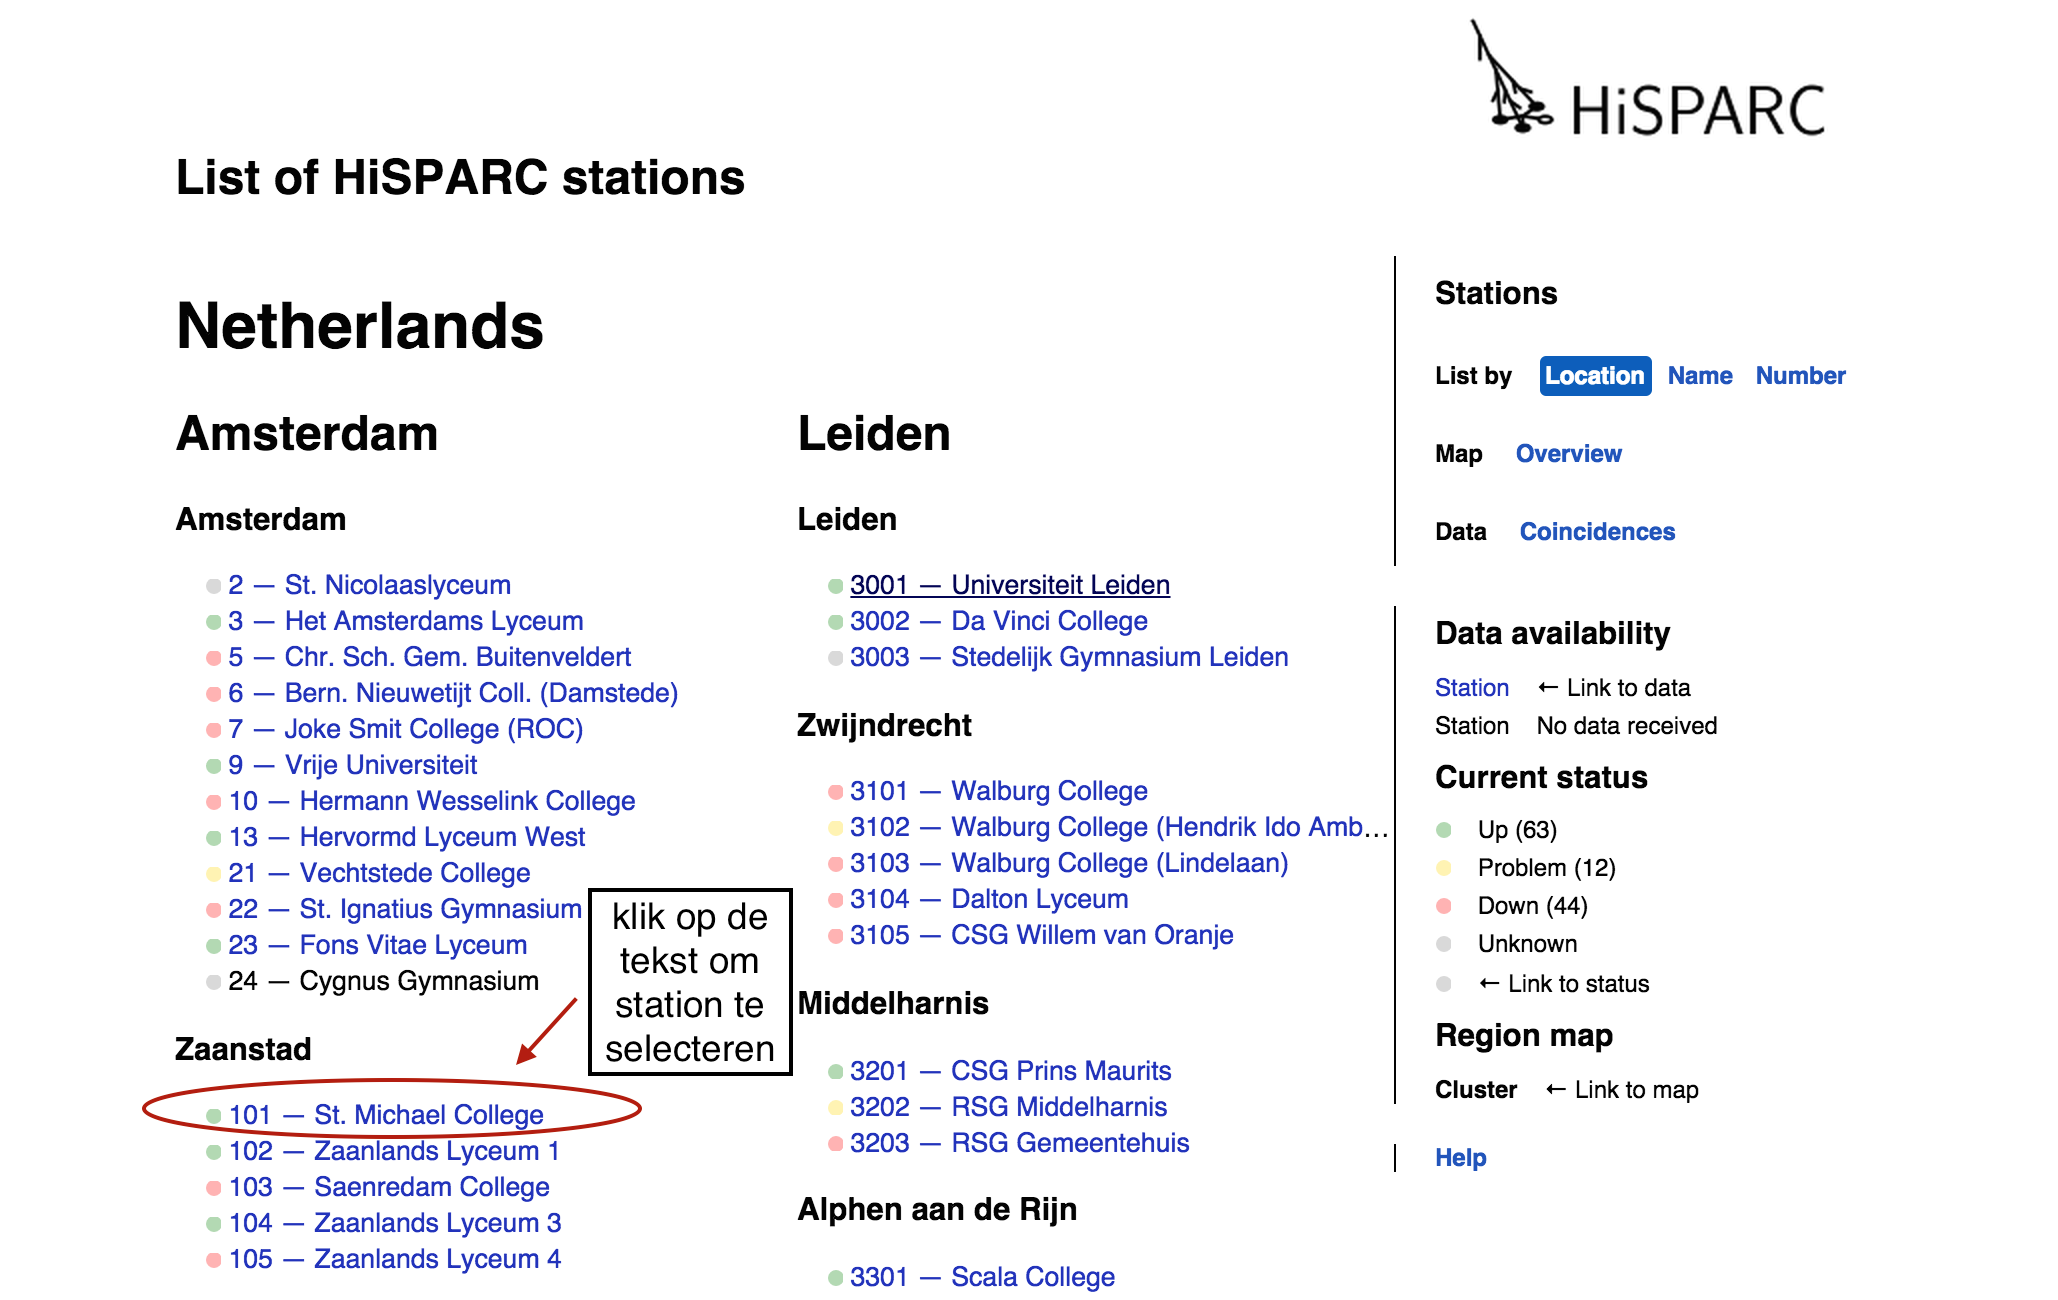
\includegraphics[scale=0.4]{overview_website}
    \caption{Weergegeven is de website \textit{http://data.hisparc.nl}. 
    Klik nu op een station om op de pagina van 
    het station te komen.}
    \label{fig:overview_website}
\end{figure}

\begin{figure}
    \centering
    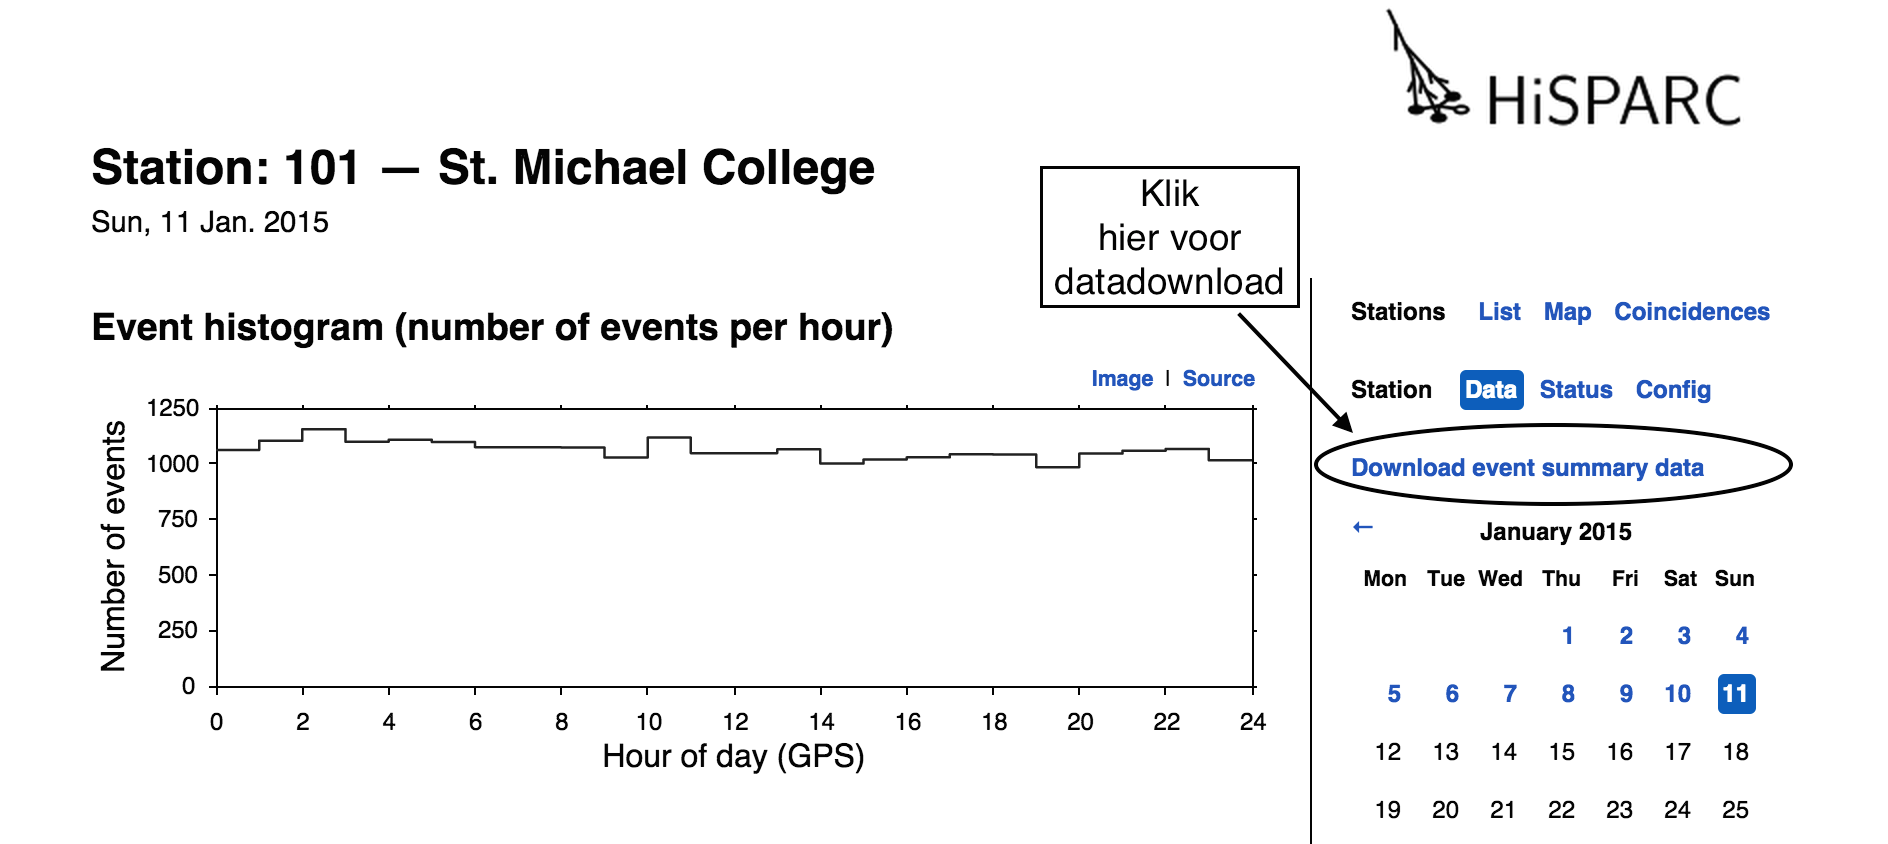
\includegraphics[scale=0.4]{data_download}
    \caption{Klik op `download event summary data', om bij het dataformulier te komen.}
    \label{fig:data_download}
\end{figure}

\begin{figure}
    \centering
    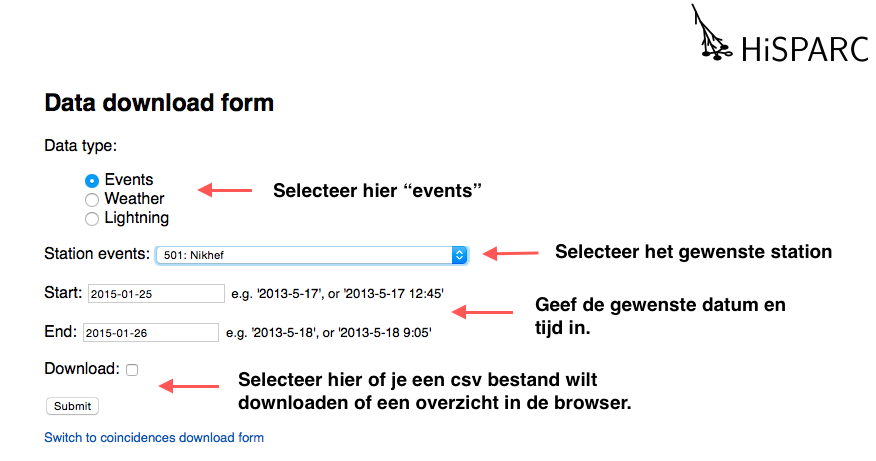
\includegraphics[scale=0.35]{data_download_form}
    \caption{Selecteer op deze site het gewenste station, de begin- en einddatum en tijd 
     en of je de data als csv-bestand of in je browser wilt hebben. Als er oefeningen met 
     het inlezen in Excel gedaan worden, dan moet je de data als csv-bestand downloaden.
     Neem de tussenposen tussen de begin- en einddatum en tijd klein (een paar uur), 
     omdat je snel heel veel data hebt. Te grote tijdsduur resulteert in grote databestanden.}
    \label{fig:data_download_form}
\end{figure}


\begin{figure}
    \centering
    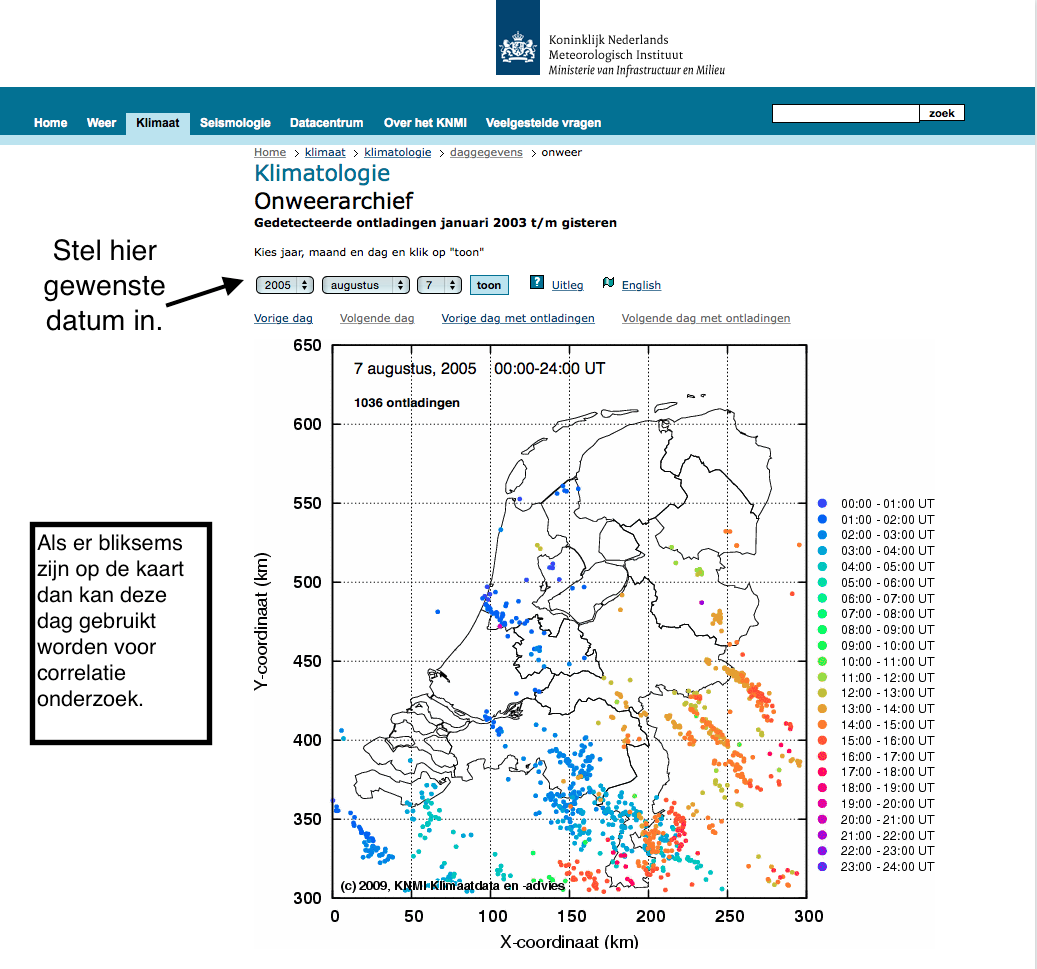
\includegraphics[scale=0.35]{KNMI_data}
    \caption{Op deze site van het KNMI (website 1) kun je snel dagen met bliksem vinden. Als een dag 
    met bliksem is gevonden, moet gecheckt worden of het \hisparc station wat in de
    buurt staat van veel bliksemontladingen, online was die dag. Zo ja, dan kan 
    er met het dataformulier zowel bliksemdata als kosmische straling events
    gedownload worden.}
    \label{fig:KNMI_data}
\end{figure}


\end{document}
